%In \S\S \ref{sec:reqt_philosophy},\ref{sec:wl_gal-clusters},\ref{sec:gc}, we
%describe our work plan and explain how we will iteratively flow down science objectives to the
%measurements to be conducted, develop observational strategies,
%simulate synthetic astronomical `truth' data and the observational
%data output (including calibration), develop a methodology for
%validating dark energy constraints, and define scientific performance
%requirements and a complete plan for the science investigation.
%Our work plan maps the six SIT tasks into the deliverables below. For each deliverable, we identify in parentheses the required tasks (numbered \textit{T 1-6} as in \S 3.1 of the WFIRST SIT call). We will also associate explicitly the sections of our proposal to the deliverables.

\begin{summary}
In our proposal, we structured our planning around a series of
deliverables numbered D1-12. We will use throughout this report the same
nomenclature and report on our progress on each of these deliverables and compare the current status with the proposed calendar visible in Figure~\ref{tab:milestones_mgt}.

In the text below, the definition of each deliverable is summarized and is followed by a status update. We compare favorably on all deliverables with one exception we discuss. We note that when discussing delivery dates, we replaced fiscal year by calendar year as it is a better match given the start of our effort after selection, in January 2016.
\end{summary}


% We will present in this detailed report our progress on these deliverables and
% illustrate that we either reached or exceeded our proposed expected milestones.

%Our work plan maps the six SIT tasks,  identified in parentheses  (numbered \textit{T 1-6} as in \S 3.1 of the WFIRST SIT call), to the deliverables below.
%For each deliverable, we identify in parentheses the required tasks.

%a given deliverable it encompasses.
%  For each
% deliverable,

%  In
% order to map our work plan into the six SIT tasks and our list of
% deliverables, we explicitly associate the subsequent sections with
% these deliverables.


%\subs{Program Milestones.} In Fig.~\ref{tab:milestones_mgt} we outline milestones for
%our effort in conjunction with the project timeline.\setlength\intextsep{-2pt}


\subsection*{(D1) Full requirements flow-down}
%============================================

\paragraph*{Deliverable:} Full requirements flow-down from the high-level science goals of the HLS galaxy clustering and weak lensing survey to detailed performance of the telescope, wide field instrument, software, operations, and data transfer.

\paragraph*{Delivery Date:} CY16, CY18

\paragraph*{Status: On schedule.} Throughout the last 2.5 years, we delivered three versions of the level 2 science requirements for both the HLSS and the HLIS. We have been updating them on request since the latest delivery.

\subsection*{(D2) Forecasts of the cosmological performance of the HLS Imaging
and Spectroscopy data sets}
%===============================================================================

\paragraph*{Deliverable:} Forecasts of the cosmological performance of the HLS Imaging
and Spectroscopy data sets, including expected constraints on dark energy,
modified gravity, neutrino masses, and inflation, from analyses that include the
measurement of the location of the Baryon Acoustic Oscillations (BAO),
Redshift-Space Distortions (RSD), galaxy power spectrum and higher order
statistics, cosmic shear, galaxy-galaxy lensing, and cluster demographics. These
forecasts incorporate realistic assessments of observational systematics and
theoretical modeling systematics, and they examine the expected constraints from
different probes individually, in concert with each other, and in concert with
expected constraints from the WFIRST supernova program, CMB experiments, and
other cosmological surveys such as DESI, LSST, and Euclid. We use our
forecasting tools to investigate trades, e.g., the impact of survey or
instrument design choices (area, depth, pixel size, spectral resolution, etc.)
on cosmological performance.

\paragraph*{Delivery Date:} CY16, CY17, CY20

\paragraph*{Status: On schedule.} We developed and updated a unique software package (\CoLi) \citep{Eifler:2014,Krause17} that enables us to jointly forecast all the WFIRST cosmological probes, including their covariance. We used this framework to conduct trade studies. We released to the community the associated WFIRST chains \href{http://www.wfirst-hls-cosmology.org/products/}{[Link]} and the code on \texttt{GitHub} \href{https://github.com/CosmoLike}{[Link]}. We are now completing a forecast paper led by co-I Eifler that will be submitted before the end of CY18. Relying on state-of-the-art methods, it includes combined forecast (weak lensing, cluster counts, galaxy redshift survey) for the notional HLSS and HLIS surveys as well as possible extensions, such as one band deep imaging survey covering the LSST footprint. In a next paper, we plan to use this package to revisit the HLSS optimization, and also to include SNe.

\subsection*{(D3) Simulated imaging and spectroscopic data sets}
%==============================================================

\paragraph*{Deliverable:} Simulated imaging and spectroscopic data sets for
testing pipeline performance and evaluating systematic biases --- e.g., from
confusion, noise, and incompleteness in images and spectra, or errors in Point
Spread Function (PSF) determination or shape measurement. These data sets will
be created with varying levels of complexity in the source catalogs and
instrumental effects, to allow isolation of individual contributions to
statistical and systematic uncertainties. Some of these artificial data sets
will be made publicly available, and some will take the form of data challenges,
where the underlying parameters are initially known only to the creators of the
data set, in the spirit of the Shear Testing Program (STEP) and Gravitational
Lensing Accuracy Test (GREAT) weak lensing data challenges \citep{Heymans2006,
Massey2007, Bridle2010, Kitching2012, Mandelbaum2015}.

\paragraph*{Delivery Date:} CY16, CY19, CY20

\paragraph*{HLIS Status: On schedule.} We implemented and maintain a
WFIRST dedicated module in the state-of-the-art image simulation
pipeline \texttt{GalSim} \citep{Rowe:2015}. We released this module to the community
\href{https://github.com/GalSim-developers/GalSim}{[Link]}. This module currently includes the following functionalities for simulating WFIRST-like images according to Cycle 7 specifications: PSF and pupil plane description, telescope astrometry, filter bandpasses, and specifications for applying detector-level modifications to observations such as reciprocity failure, quantization, persistence, nonlinearity, and interpixel capacitance. This module was described in \cite{Kannawadi2016}. Near term extensions will include implementation of a more realistic persistence model based on ongoing detector characterization tests. The GalSim implementation is supplemented by a simulation wrapper \href{https://github.com/matroxel/wfirst_imsim/}{[Link]} to create realistic image simulations of simulated HLS realisations, including appropriately simulated dither sequences (taken from a full 5-year tiling simulation with observing constraints and overheads) and appropriate galaxy and star photometry, redshift, and morphology distributions. We have not released images directly generated by this code yet, but it is the backbone of our efforts to validate imaging requirements for weak lensing and the new deliverable dedicated to produce joined WFIRST-LSST simulations described in \S\ref{sec:joint_simulations}. A paper describing this simulation package and initial uses by the SIT is in preparation, which will include a public release of images simulating a part of the five-year HLS imaging.

\paragraph*{HLSS Status: On schedule.} We were initially planned to support the mock observation generated by the SOC but since this task was removed from their charge, the SIT took over the full effort. We are making active progress and summarize below the current status and plan.
\begin{itemize}
\item We adapted and modified James Colbert's WFIRST grism simulation so that it can easily be used with any input catalog. James Colbert is now a collaborator in our SIT and Anahita Alavi (IPAC) is leading this task. Completed Summer 2018)
\item We created input catalogs based on Alex Merson and Andrew Benson's \texttt{Galacticus} semi-analytical galaxy evolution simulations. To be completed before Sping 2019.
\item We will create 4 sq. deg. WFIRST grism simulations, and send it to Science Center (assigned by the WFIRST Project Office) for redshift and flux measurements, to determine the completeness and purity of WFIRST GRS. To be completed before Spring/Summer 2019.
\item We will release to the community the 4 sq. deg. grism simulations and provide support. To be completed before the end of Summer 2019.
\item We will then create 2000 sq. deg. simulated WFIRST GRS galaxy catalog, calibrated with grism simulations, for studying the modeling of systematics and the realistic forecasting of dark energy and cosmological parameter constraints. To be completed before Spring 2020.
\item We will then prepare the simulated data for public release through summer 2020 and release it with documentation before the end of FY20.
\end{itemize}


\section*{(D4) Proto-type imaging and spectroscopic pipelines}
%=============================================================

\paragraph*{Deliverable:} Proto-type imaging and spectroscopic pipelines,
including weak lensing shape measurement and galaxy redshift measurement, tested
against the above artificial data sets. These proto-type pipelines will provide
building blocks for development of full pipelines during the implementation
phase, and they will allow us to sharpen definitions of software requirements
and to identify challenges to and strategies for meeting these requirements.

\paragraph*{Delivery Date:} CY18

\paragraph*{HLIS Status: Delayed.} We have adapted so far adapted tools from other state-of-the-art data pipelines, such as HSC or DES. Once we have received final instructions from the Project Office on this matter, we will assemble the relevant documents based on this experience.

\paragraph*{HLSS Status: Delayed.} We started to develop dedicated quick tools that
will allow us to build and evaluate a GRS pipeline. This software package allows us to make quick forecasts on basic dark energy parameters from higher order statistics, including power spectrum and bispectrum multipoles. This light and agile software package will be the backbone of our GRS proto-pipeline effort. Once we have received final instructions from the Project Office on this matter, we will assemble the relevant documents based on our experience with BOSS.

\section*{(D5) Calibration strategies}
%=====================================

\paragraph*{Deliverable:} Calibration strategies for photometry, shape
measurement, spectroscopy, and redshift completeness. Evaluation of the expected
performance of these strategies against the science requirements. The
requirement on knowledge of the dark current and the calibration approaches are
fully defined, based on analysis done during the dark filter trade (October 2016
-- February 2017).

\paragraph*{Delivery Date:} CY17, CY18

\paragraph*{Status: On schedule.} We contributed extensively to the WFIRST WFI Calibration Plan which is still in flux. This includes extensive quantitative analysis of proposed calibration techniques. We have also been testing some of the calibration techniques for gain, inter-pixel capacitance, and non-linearity (including the brighter-fatter effect) using laboratory data (taken at the GSFC Detector Characterization Laboratory). This is informing us on which techniques are working well on H4RG-10 data and where there are challenges in achieving repeatability or agreement between methods at the level expected from ``$1/\sqrt N$'' arguments. We have been in particular looking at the impact of our current best estimate of detector performances on the required calibration frequency. We are actively participating in Calibration Working Group discussions on what ground tests are required for calibration.


\section*{(D6) A strategy for the determination and calibration of photometric redshifts}
%=====================================================

\paragraph*{Deliverable:} A strategy for the determination and calibration of
photometric redshifts using WFIRST data and anticipated external data (e.g.,
LSST optical photometry), and defining ground-based data that are needed to
implement this strategy (e.g., spectroscopic training sets, large redshift
surveys for calibration via cross-correlation). Evaluation of the impact of
remaining photometric redshift uncertainties on statistical and systematic
errors in weak lensing and clustering analyses.Definition of requirements for
WFIRST photometric redshifts informed by this strategy and evaluation.

\paragraph*{Delivery Date:} CY18, CY19

\paragraph*{Status: On schedule.} We made substantial progress by co-leading a
large dedicated spectroscopic observation program (C3R2), generating mock WFIRST
and LSST observations based on HST CANDELS data (released to the community here
\href{http://www.wfirst-hls-cosmology.org/products/}{[Link]}), by devising
calibration strategies based on Self-Organized Maps
\citep{Masters2017,Hemmati:2018}, and by studying the importance of the Integral
Field Channel (IFC) to calibrate photometric redshifts. We are currently
studying the use of a low resolution prism to replace the IFC following a
request from the Project Office. We also studied the potential use of JWST, both
for direct observations and in parallel modes, and have been in touch with the
STSci director, the NIRSpec team, and the JWST project about this possibility.
We have developed a series of simulations based on CANDELS that indicate NIRSpec
in a pure parallel mode using a grid of slits could potentially replace the
capability of the IFC for redshift calibration.  We have confirmed with the
NIRSpec team this is technically possible and the JWST project has indicated it
should be relatively easy to implement. A report outlining the findings is being
written for consideration by the JWST project. We have also begun to explore the
use of cross-correlations to calibrate the redshift distributions by applying
\texttt{the-wizz} \citep{Morrison:2017} to existing data sets in COSMOS and SXDS
as well as simulations.  Our focus is currently on determining the requirements
on the number-densities at higher-redshifts (z$>$1) and the effects of having
biased and variations on that bias in the spectroscopic samples.  The first
paper detailing applications of this method to high-redshift sub-mm sources, a
traditionally difficult and outlier population, is being finalized.

\begin{figure}
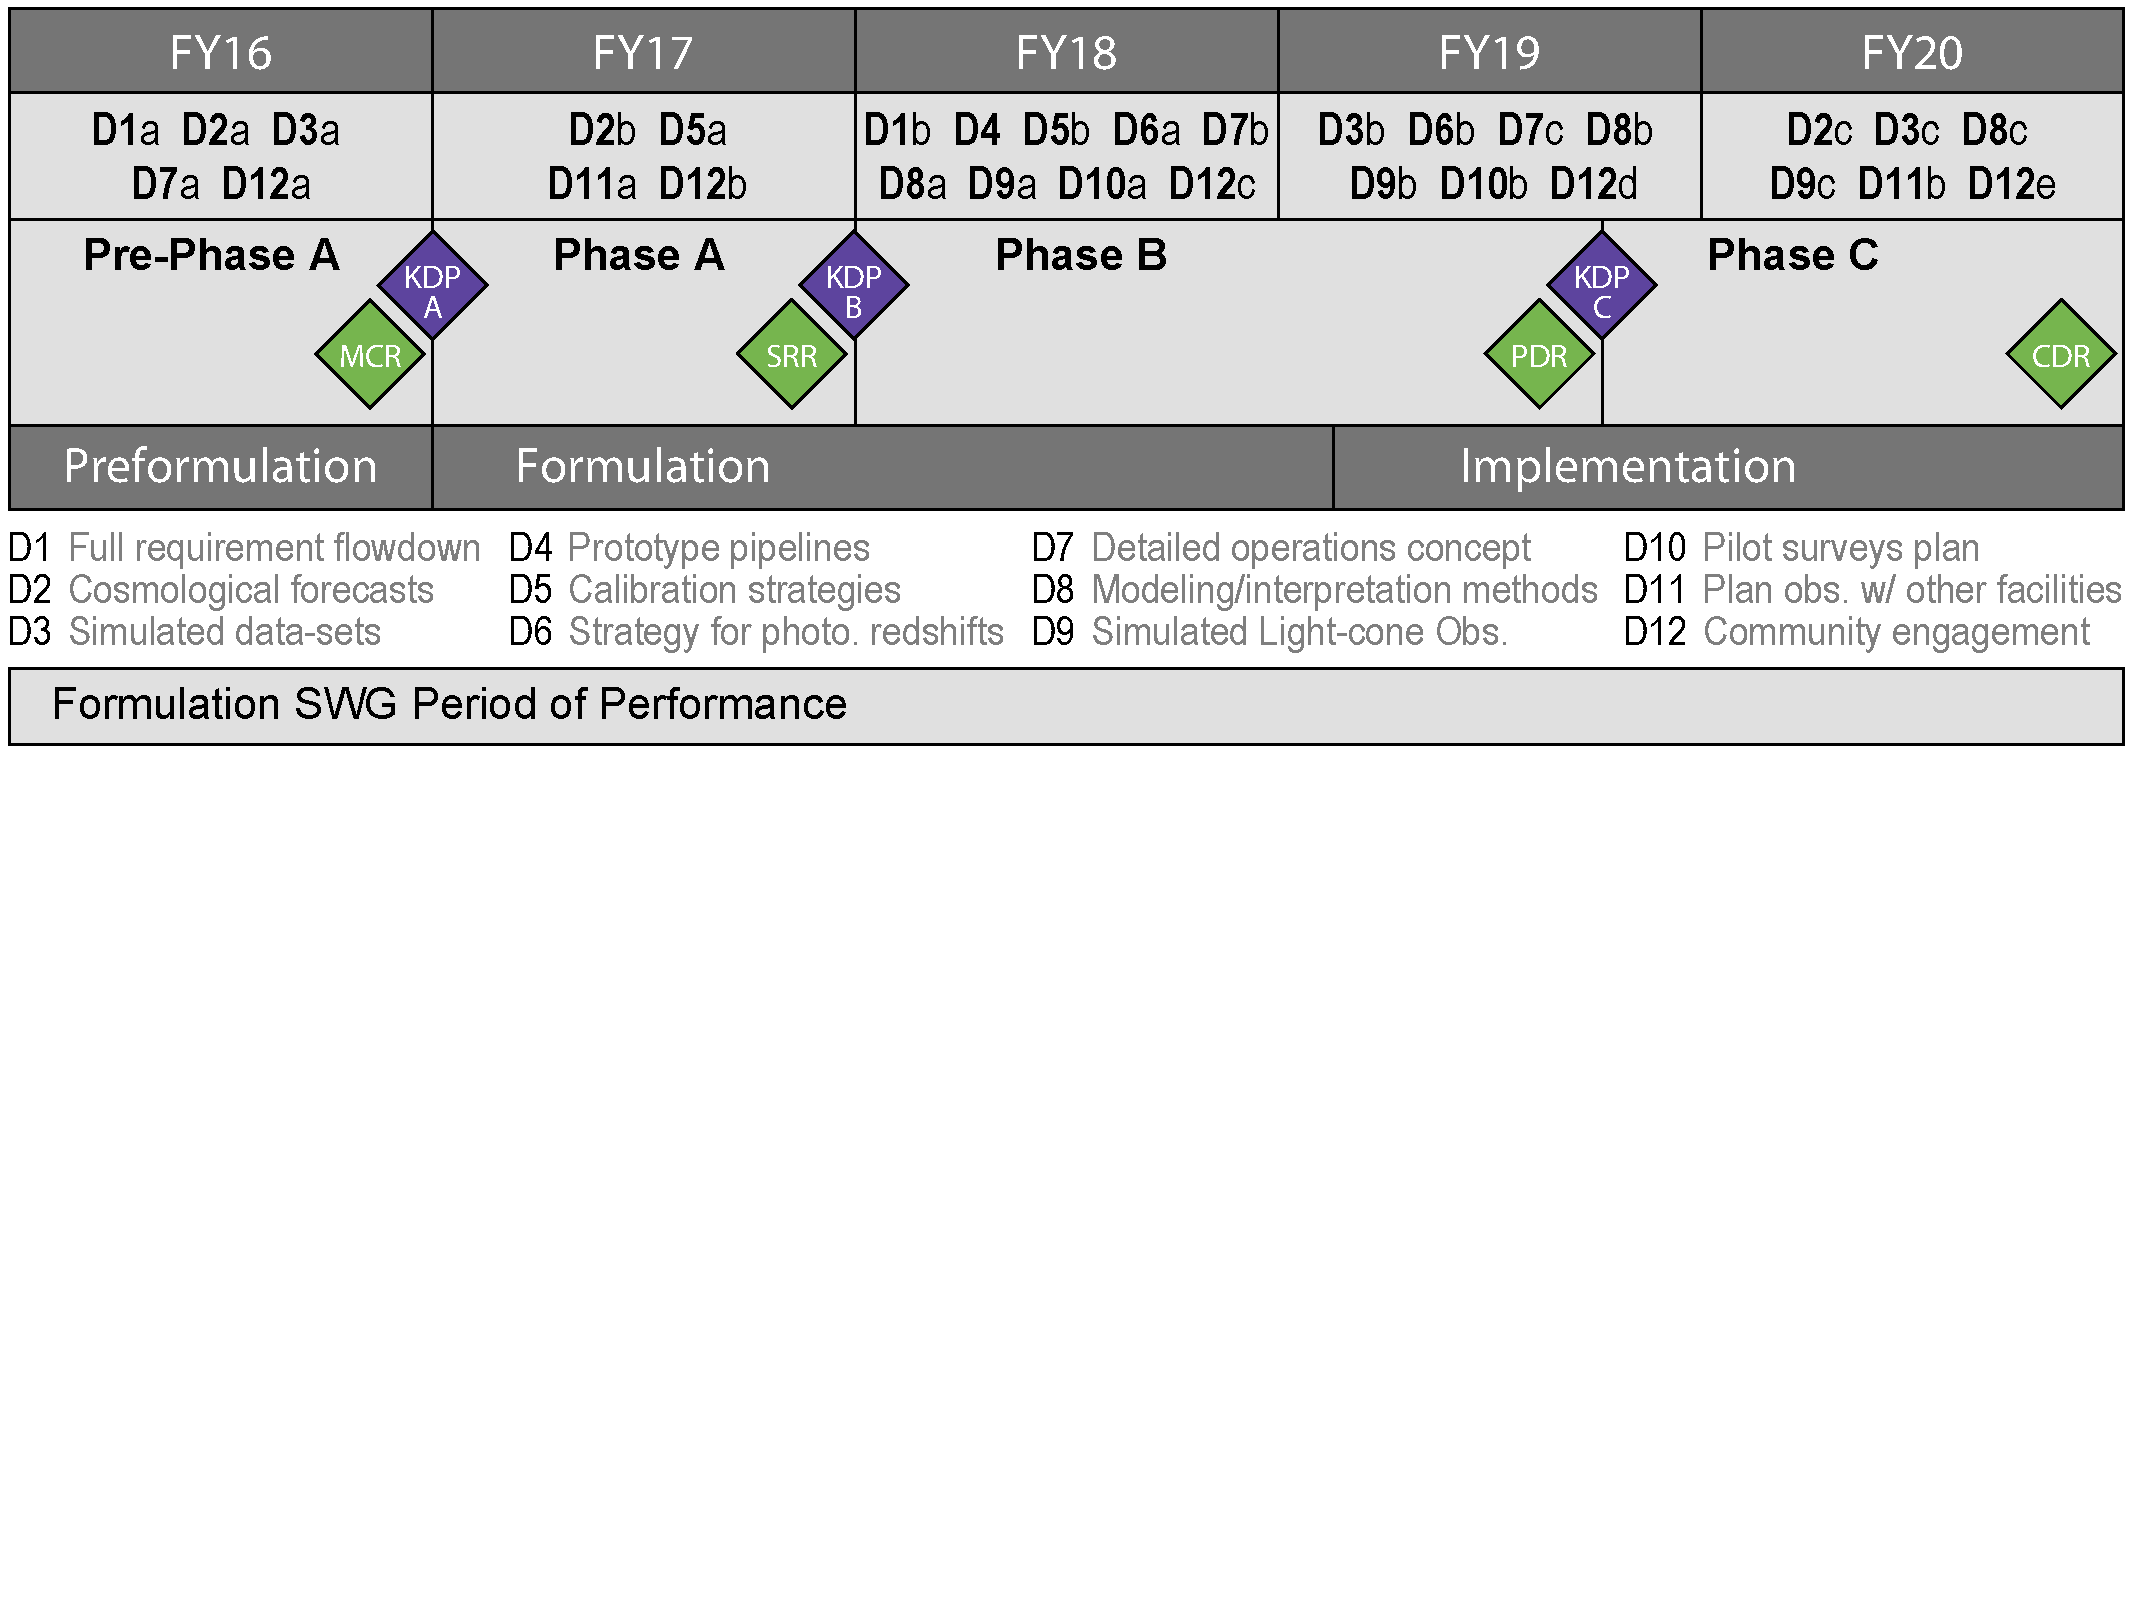
\includegraphics[width=0.99\textwidth]{Plots/wfirst_milestones_v2.pdf}
\caption{Our proposed deliverable schedule in concordance with the WFIRST
project timeline as displayed in the WFIRST SIT call \S 3.2. Deliverables that
are made in multiple stages are labeled (a, b and c) and appear in multiple
years. This figure is taken from our original proposal and the schedule has in
fact shifted since our investigation started on January 2016, thus well into
FY16. In the text, we thus changed FY into CY.} \label{tab:milestones_mgt}
\end{figure}


\section*{(D7) A detailed operations concept for the HLS Imaging and Spectroscopy
program}
%=================================================================================

\paragraph*{Deliverable:} A detailed operations concept for the HLS Imaging and Spectroscopy program, extending the work presented in SDT13 and SDT15.

\paragraph*{Delivery Date:} CY16, CY18, CY19

\paragraph*{Status: On schedule.} In collaboration with the relevant WFIRST WG, which we are co-leading, we delivered to the project multiple detailed updates to the operation concept and propagated it into image simulations and forecasts.


\section*{(D8) Development of methods for modeling and interpreting the cosmological
measurements anticipated from WFIRST}
%==================================================================================

\paragraph*{Deliverable:} Development of methods for modeling and interpreting the cosmological measurements anticipated from WFIRST. Determination of the effects of non-linear gravitational clustering, realistically complex relations between the
galaxy and dark matter distributions, and the influence of the baryon
component on matter clustering. The study of techniques to
remove systematic biases, e.g., by marginalization over nuisance
parameters. Utilization of cosmic shear, galaxy-galaxy lensing, cluster mass functions and cluster weak lensing, BAO, RSD, the galaxy
power spectrum, and higher order statistics for galaxy clustering, weak
lensing, and various combinations. Identification of areas where
further improvements of theoretical modeling would significantly
enhance the cosmological return from WFIRST.

\paragraph*{Delivery Date:} CY18, CY19, CY20

\paragraph*{Status: On schedule.} We made progress on several fronts summarized below.

\begin{itemize}

\item {\bf Voids.} We started testing the void finding procedure on the first
WFIRST OIII mock galaxy catalog (see mock description below). We tested mask
effects by simulating a simplistic mask and we cut the mock to simulate the area
observed by WFIRST ($\simeq$ 2200 sq. degrees). This is extremely relevant for
voids as we remove voids that intersect boundaries, hence it allows to estimate
how the voids statistic is impacted. From the [OIII] catalog we obtain $\simeq$
10500 voids. We are starting work to fit the theoretical void size function
prediction to voids from this catalog (as void size function has been shown to
be a relevant tool to constrain the dark energy equation of state, see
\cite{Pisani2015}). This involves testing theoretical models on current void
catalogs from data, and considering different models (mainly the model from
\cite{Sheth2004}, and the Vdn model from  \cite{Jennings2013}. This work is also
important to make the void abundance forecasts for WFIRST as realistic and
reliable as possible. As soon as the $H\alpha$ mock will be available we also
plan to run the void finding procedure on that catalog. The $H\alpha$ catalog
will be particularly interesting to use for void science because it will allow
to confirm the huge power of WFIRST in capturing more voids and their detailed
substructure with a denser galaxy distribution.

\item {\bf Emission line separation.} At high redshifts, the primary target will
be the [OIII] line. This line and H$\beta$ are very close in wavelength and
hence the photo-$z$ could be unable to distinguish them reliably. Confusing them
might be problematic because misidentifying an H$\beta$ emitter as [OIII] will
cause a difference in the inferred radial position of about $90$ Mpc/$h$, which
is very close to the BAO scale. Therefore, the confusion can introduce
systematic errors in the BAO analysis. We created a WFIRST-like catalog
containing both [OIII] and H$\beta$ emitters, where the latter are placed at the
wrong redshift, as misidentified as [OIII]. This catalog has been generated from a light cone simulation and is public available at
[\href{http://www.wfirst-hls-cosmology.org/products/}{Link}]. Using the catalog,
we are studying the impact of this effect on the BAO peak and the resulting BAO
analysis.

\item {\bf Galaxy cluster modeling.} The high number density of background galaxies of WFIRST is expected to revolutionize the field of weak lensing for galaxy clusters.  With this unprecedented signal-to-noise ratio, we need accurate modeling for the mass density profiles of galaxy clusters, as well as their covariance matrices, at all scales. To this end, we use cosmological N-body simulations to improve the analytical model for lensing signals and covariance matrices.  Combining large-volume light-cone ray-tracing simulations with small-volume high-resolution simulations, we quantify the gravitational lensing effect from large-scale structure and from small-scale non-linearity. With this improved modeling, we will soon provide (1) a robust forecast for an optimal, unbiased cluster data analysis method; and (2) a user-friendly software package for accurately calculating the signal and covariance matrices of cluster weak lensing.

\item {\bf Systematics mitigation at the likelihood level.} Residual uncertainties in observational systematics (shear calibration, photo-z calibration) and astrophysical systematics (galaxy bias, galaxy intrinsic alignment, baryonic feedback and cooling processes) need to be accounted for in the likelihood analysis. We have implemented corresponding models into \CoLi, tested them in simulated likelihood analyses and on data from precursor surveys. We explored joint analyses of multiple cosmological probes \citep{Krause17,ske17} and quantified the cosmological information in the presence of various systematics parameters and systematics mitigation strategies. We explored the impact of individual systematics such as the impact of baryons and intrinsic alignment \citep{ekd15, keb16,hem18} and implemented corresponding models for the survey specifications of WFIRST. We have also tested our modeling abilities on precursor data sets of WFIRST most importantly the Dark Energy Survey (DES) \citep{kez17, DES17}. The implementation relies on massively parallelized computation of fine-tuned look-up tables with a targeted sub-second run-time per point in parameter space. Given the large number of parameters describing systematic effects in future LSS analyses this efficient computation ensures acceptable turnaround times. In particular, it allows for the large number of simulated likelihood analyses that are needed to optimize future surveys.

\end{itemize}


%have not started to work on this deliverable yet besides generating realistics mock observations (\S \ref{sec:light-cone}).

\section*{(D9) Simulated light-cone observations}
%================================================

\paragraph*{Deliverable:} Simulated light-cone observations based on
cosmological simulations for guiding this methodology development and testing
its performance. Most of these data sets will be at the level of galaxy redshift
and shape catalogs rather than the pixel-level imaging and spectroscopy
simulations described above.  They will incorporate varying degrees of
complexity regarding galaxy bias, redshift evolution, survey geometry, and
observational systematics such as incompleteness, shape measurement errors, and
photometric redshift biases.  Many of these artificial data sets will be made
publicly available, and some will take the form of data challenges, where the
underlying parameters are initially known only to the creators of the data set.

\paragraph*{Delivery Date:} CY18, CY19

\paragraph*{Status: On schedule.} We started assembling multiple light-cone
observations dedicated to GRS, but also WL+GRS. We created and released a WFIRST
[OIII] mock galaxy catalog from a light cone simulation
\href{http://www.wfirst-hls-cosmology.org/products/}{[Link]}. The simulation
contains about 3 billion galaxies over 10,313 sq. degrees and up to redshift
2.3. Each galaxy contains its own spectral energy distribution which is
generated to fit the most updated luminosity function and color evolution
measurements. The catalog contains galaxies in the redshift range 1 to 2.3, with
a number density and redshift distribution that mimic the ones forecasted for
the WFIRST. A companion paper is being finalized (Massara et al.).

This mock catalog is a first pass and partially meets the WFIRST requirements.
It does not include yet the primary WFIRST tracer (H$\alpha$) and the [OIII] line
is modeled at redshifts below the primary range of $z=2-3$ for WFIRST [OIII]. A
light cone simulation used for grism simulation is also been generated using a
physically-motivated galaxy formation model implemented in the
\texttt{Galacticus} software (see D3) \citep{Benson2010}. Preliminary mock
catalogs have already been constructed and have been used to predict the number
density of H$\alpha$-emitting galaxies \citep{Merson2018}. These mocks can be
made publicly available if needed. We are in the process of building updated
mock catalogs using \texttt{Galacticus} that will include spectral energy
distributions (SEDs) for each galaxy, which will be used to construct grism
simulations (see D3). These mock catalogs are being built using the Millennium
Simulation \citep{Springel05}, which we note lacks sufficient volume for WFIRST.
However work is also underway to apply \texttt{Galacticus} to much larger volume
simulations.

We also generated light-cone simulations using the approximate method ICE-COLA \citep{Izard2016,Izard2018}. This method lets one to trade accuracy at small scales in order to gain large speed-up factors in the computations, and this results optimal for producing massive ensembles of simulations. We currently have 500 light cone simulations of the dark matter distribution and we developed an efficient pipeline based on Ghost \citep{Bull2017} to turn these into galaxy catalogs. The resulting mock catalogs contain $\sim$ 200M galaxies over the whole sky in the redshift range from 0 to 1.4, have photometry in the u,g,r,i,z  bands (we plan to implement WFIRST bands in the future) and weak-lensing quantities. Therefore, they are suitable for covariance studies for the GRS+WL. At the moment of this report, we have run the galaxy pipeline in only one realization, which has been used for testing and validation (Izard et al. in prep., where we also use the catalogs to do a study of some observational systematics), and we plan to run the pipeline to the whole ensemble of 500 light cones in CY19.

\section*{(D10) Pilot survey proposals with associated figures of merits}
%========================================================================

\paragraph*{Deliverable:} Pilot survey proposals with associated figures of merits, to be executed during the first months of WFIRST operations. These would become
part of the final dark energy data set but also pin down remaining astrophysical
or instrument performance uncertainties at the level needed to optimize the HLS.
We will develop the figures of merit required to quickly assess the data-quality
and make operational decisions regarding the cosmological surveys.

\paragraph*{Delivery Date:} CY18, CY19

\paragraph*{Status: On schedule.} This activity has not fully started yet beyond discussions of the deep fields, in conjunctions with the other SITs and other major observational efforts during our community workshop (see D12). Team members were key participants in a Princeton workshop dedicated to deep fields. This is directly relevant as the deep field are likely to be part of the pilot program. We are planning for the coming year CY19 to define exactly what we want to get out of a pilot survey (e.g., actual in-flight observatory performance, initial estimates of the clustering amplitude of source populations, etc.).

\section*{(D11) A prioritized program of observations from other facilities}
%============================================================================

\paragraph*{Deliverable:} A prioritized program of observations from other facilities
ground and space-based, needed to calibrate or finalize strategy decisions on
the WFIRST dark energy program.

\paragraph*{Delivery Date:} CY17, CY20

\paragraph*{Status: On schedule.} Members of our SIT are leading an ambitious spectroscopic observations campaign (C3R2) aiming at calibrating photometric redshifts
for WFIRST and other surveys. Members of our team are leading a major
observational program on Spitzer (the Spitzer Legacy Program (SLS)) to prepare for WFIRST and others. We are currently writing a LSST Cadence White paper to address the specific requirement on LSST from a WFIRST HLS point of view  \href{https://www.lsst.org/call-whitepaper-2018}{[Link]}. We are also participating in a LSST Cadence white paper focused on Deep Fields. We investigated proposing for JWST time to calibrate the photometric redshift of faint red galaxies \citep{Hemmati:2018}. We also studied the potential use of JWST, both for direct observations and in parallel modes, and have been in touch with the STSci director, the NIRSpec team,  and the JWST project about this possibility.  We have developed a series of simulations based on CANDELS that indicate NIRSpec in a pure parallel mode using a grid of slits could potentially replace the capability of the IFC for redshift calibration.  We have confirmed with the NIRSpec team this is technically possible and the JWST project has indicated it should be relatively easy to implement.  A report outlining the findings is being written for consideration by the JWST project.

The use of Subaru PFS and HSC to mitigate the redshift calibration problem has
also been studied.  Preliminary results indicate the Subaru PFS spectrograph
could obtain redshifts to most of the faint WFIRST weak lensing samples in
$\simeq$20-100h exposures if it is not systematics limited at these long
exposure times.  However, this level of systematics control has not been
demonstrated for a fiber spectrograph.  Early deep observations with PFS should
demonstrate if this type of observation is feasible or not.  Since the number of
high-resolution spectra obtainable are also naturally limited we have also been
considering the use of R$\simeq$20-40 intermediate band imaging on HSC (along with the
possibility of the low-resolution prism) to constrain the range of possible
galaxy spectra.  While this approach does not provide high-quality redshifts, it
does provide detailed information on rare catastrophic outlier populations.  The
potential presence of these objects is the driving requirement for obtaining
large numbers of spectra, so alternative methods that mitigate them has the
potential to significantly reduce the spectroscopic calibration burden.  We are
in the process of developing metrics for this technique and expect some early
results in 2019.

\section*{(D12) Broad engagement with the cosmological community}
%=================================================================

\paragraph*{Deliverable:} Broad engagement with the cosmological community, through
workshops, talks, publications, and public release of codes and artificial data
sets, with the goals of (a) building awareness of and broad support for the
WFIRST dark energy program and (b) inspiring the community to develop methods
and carry out investigations that will maximize the cosmological return from
WFIRST.

\paragraph*{Delivery Date:} CY16-CY20

\paragraph*{Status: On schedule.} We organized in September 2016 our first community workshop in Pasadena. It was dedicated to enabling the scientific synergies between WFIRST HLS and LSST DESC. Our second community workshop dedicated to synergies between WFIRST HLS and other surveys happened in February 2018 \href{http://www.wfirst-hls-cosmology.org/workshops/}{[Link]}. We surveyed, reviewed, and discussed synergies with major surveys of the 2020s, such as LSST, Euclid, Spitzer, JWST, HSC/PFS, SKA and ngVLA, CMB S4, and eROSITA. We discussed the best way to enable new science with the WFIRST HLS. This workshop was instrumental in converging on a list of joined deep fields accross Euclid, LSST, and WFIRST. A future workshop will happen in CY19. The focus is still to be determined.

%\Oli{Peter, please add anything I might have forgotten.}
